% ------------------------------------------------------------------
% Achieved cache size: Pareto figure + achieved-compression table.
% Source: experiments/results/pareto_oracle_analysis.md
% Figure regenerated by: experiments/scripts/pareto_oracle_analysis.py
% ------------------------------------------------------------------

\begin{figure}[t]
  \centering
  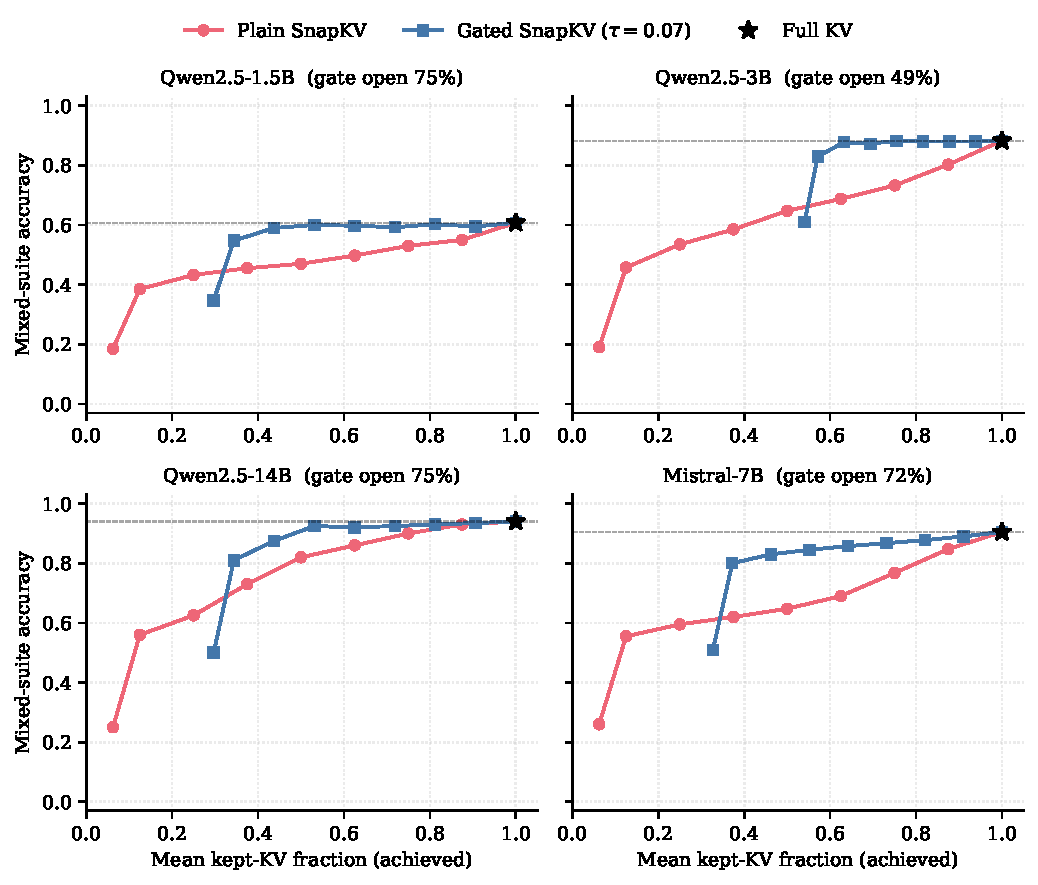
\includegraphics[width=0.92\linewidth]{figs/pareto_gated.pdf}
  \caption{Accuracy vs.\ \emph{achieved} kept-KV fraction (mean over inputs of
  $n_{\text{kept}}/T$) on the mixed 4K suite (NIAH-MK3 + VT + FWE + QA\_1),
  SnapKV. Because the gate falls back to the full cache when it closes, gated
  points sit at larger kept-KV than their nominal budget; the honest comparison
  is at matched achieved cache size. For every target kept-KV fraction
  $\gtrsim 1/3$ (Qwen3B: $\gtrsim 0.57$) the gated curve is the Pareto
  frontier, by up to $+19$pp over plain at equal cache size; at the most
  aggressive nominal budget ($b=0.0625$, leftmost gated point) the gated point
  is dominated by plain eviction at a matched cache size, and $\tau=0.07$
  caps achievable compression at $1-\text{open-fraction}$ of the cache
  ($0.25$--$0.51$ across models). All gated results use the post-hoc
  $\tau=0.07$ reconstruction (Appendix~\ref{app:repro}); the reconstruction
  reproduces the stored gated outcomes exactly on the three runs executed at
  $\tau=0.07$.}
  \label{fig:pareto-gated}
\end{figure}

\paragraph{What cache size does the gate actually deliver?}
Table~\ref{tab:matrix} compares plain and gated at matched \emph{nominal}
budget, but the gate's full-KV fallback means the two arms hold different
amounts of cache: the achieved kept-KV fraction at nominal budget $b$ is
approximately $(1-p_{\text{open}}) + p_{\text{open}}\,b$, where
$p_{\text{open}}$ is the gate-open fraction
(Table~\ref{tab:achieved-compression}). Re-plotting accuracy against achieved
kept-KV (Figure~\ref{fig:pareto-gated}) shows that gating is not a free win at
every cache size but a strict improvement of the accuracy--memory frontier over
a wide range: for any target cache size above roughly one third of full KV, the
gated evictor delivers $3$--$19$pp higher accuracy than plain SnapKV at the
\emph{same} achieved kept-KV, on all four models. Below that range the picture
inverts --- at nominal $b=0.0625$ the gated mixture (near-floor accuracy on
gate-open inputs, full cache on the rest) is dominated by uniform plain
eviction at a matched cache size, and $\tau=0.07$ bounds the achievable
compression at $1-p_{\text{open}}$ (so the deployment delivers
$3.1$--$3.4\times$ memory reduction at the nominal-$16\times$ operating point
on Qwen-1.5B/14B and Mistral, and $1.8\times$ on Qwen-3B). The correct claim is
therefore: \emph{gating moves the frontier up wherever moderate compression is
the target, and saturates --- by design --- where extreme compression is
demanded.} Against a per-input oracle that picks the better of eviction and
full KV for every input, the $\tau=0.07$ gate recovers $60$--$85\%$ (mean
$69\%$) of the available headroom on the four-model matrix, almost entirely via
task-level protection of the capacity-bound anchor.

\begin{table}[t]
\centering
\caption{Achieved compression of the gated deployment at $\tau=0.07$ (SnapKV,
4K mixed suite). Kept-KV is the mean over inputs of the retained cache
fraction; ``grid mean'' averages the eight nominal budgets of
Table~\ref{tab:matrix}. Plain SnapKV keeps exactly the nominal fraction
($0.0625$ at $b=0.0625$; grid mean $0.453$). The gate-open fraction is a
per-input property, independent of $b$, and sets the compression floor
$1-p_{\text{open}}$.}
\label{tab:achieved-compression}
\begin{tabular}{lccccc}
\toprule
 & & \multicolumn{3}{c}{gated kept-KV fraction} & compression \\
\cmidrule(lr){3-5}
Model & $p_{\text{open}}$ & $b{=}0.0625$ & $b{=}0.25$ & grid mean & @ $b{=}0.0625$ \\
\midrule
Qwen2.5-1.5B & $0.75$ & $0.297$ & $0.437$ & $0.584$ & $3.4\times$ \\
Qwen2.5-3B   & $0.49$ & $0.541$ & $0.632$ & $0.728$ & $1.8\times$ \\
Qwen2.5-14B  & $0.75$ & $0.297$ & $0.437$ & $0.584$ & $3.4\times$ \\
Mistral-7B   & $0.72$ & $0.327$ & $0.462$ & $0.602$ & $3.1\times$ \\
\bottomrule
\end{tabular}
\end{table}
